Obsahem následující kapitoly je popis vla\-stní implementace nástroje pro sprá\-vu ZFS. Pozornost je věnována především spolupráci jednotlivých vrstev aplikace, stručnému popisu hlavních tříd a integraci aplikace do operačního systému Solaris.
\section{Python}
Než začneme s~implementací, je nutné si ujasnit v~jakém jazyce budeme aplikaci psát.

V~operační systému Solaris interpretuje příkazovou řádku shell. ZFS je součástí Solarisu a shell nám dovoluje využívat jeho rozhraní, které je dostupné právě z~příkazové řádky. Z~počátku se tedy možnost skriptování v~shellu zdála jako dobrá volba. Nicméně shell nám nedovoluje využívat výhody objektového programování, protože nepodporuje třídy. To je v~rozporu s~naším návrhem, který využívá objektové architektury MVC.

Proto sáhneme po skriptovacím jazyku Python, který nám umožní implementaci objektově orientované architektury MVC.
\section{HTTP Server}
Při návrhu aplikace jsme zvolili webové rozhraní. Pro implementaci tohoto řešení budeme muset zvolit nějaký webový server, který nám bude zprostředkovávat komunikaci mezi naší aplikací a webovým klientem (prohlížečem). Od našeho webového serveru budeme požadovat podporu HTTPS protokolu a možnost autentizace uživatelů pomocí metody Basic protokolu HTTP.
    \subsection{Implementované řešení}
    Mezi nejznámější a nejrozšířenější zástupce webových serverů patří například \emph{Apache}. Tato komplexní implementace webového serveru by jistě dokázala splnit všechny požadavky, které požadujeme. Nevýhodou této volby je však zbytečná obsáhlost a nutnost složitější konfigurace. Z~tohoto důvodu zvolíme vlastní řešení webového serveru, které bude přesně odpovídat požadavkům aplikace.
    \subsection{Vlastní řešení webového serveru}
    Implementace vlastního řešení webového serveru bude využívat dvou standardních knihoven jazyka Python a bude se skládat z~následujících tříd:
    \begin{itemize}
      \item \verb|WzfsadmServer|
      \item \verb|WzfsadmRequestHandler|
      \item \verb|Authenticator|
    \end{itemize}

    Součástí těchto tříd bude i implementace navržených bezpečnostních opatření.
    \subsubsection{Třída WzfsadmServer}
    Třída \verb|WzfsadmServer| reprezentující vlastní webový server, bude potomkem tříd \verb|TCPServer| a \verb|ThreadingMixIn|, které jsou součástí standardní knihovny \verb|SocketServer| \cite{socketserver} jazyka Python. To znamená, že zdědí metody obou rodičovských tříd a bude tyto metody moci využívat. Dále tato třída bude implementovat šifrování komunikačního kanálu pomocí knihovny \verb|ssl|.

    Hlavním úkolem této třídy bude poslouchat příchozí spojení na předem stanoveném síťovém rozhraní a portu. V~okamžiku připojení klienta k~serveru dojde k~vytvoření instance třídy \verb|WzfsadmRequestHandler|, která bude implementovat hlavní komunikaci pomocí HTTP protokolu. Na této úrovni jsme schopni filtrovat IP adresy, které se k~serveru budou moci připojovat. V~hlavním konfiguračním souboru serveru budeme schopni stanovit seznam IP adres, které se serverem budou moci komunikovat.

    Aby bylo možné využít šifrování pomocí knihovny \verb|ssl|, budeme muset vytvořit privátní klíč pro šifrování a certifikát, kterým se server bude identifikovat. Tuto dvojici můžeme vytvořit například pomocí nástroje \verb|openssl|. Cestu k~souborům s~klíčem a certifikátem můžeme explicitně určit v~hlavním konfiguračním aplikace.

    Ke spuštění serveru stačí vytvořit instanci třídy \verb|WzfsadmServer|, které předáme port a adresu síťového rozhraní a následně na této instanci zavolat metodu \verb|serve_forever()|. Od této chvíle bude server naslouchat na stanovené adrese a portu dokud nebude ukončen.

    \subsubsection{Třída WzfsadmRequestHandler}
    Hlavní součástí webového serveru je zmíněná třída \verb|WzfsadmRequestHandler|. Tato třída je potomkem třídy \verb|BaseHTTPRequestHandler|, která je součástí standardní knihovny \verb|BaseHTTPServer| a zajišťuje komunikaci pomocí HTTP protokolu. Součástí této třídy bude i implementace autentizační metody Basic.

    Při ověřování požadavku ověříme, jestli klient poslal autentizační údaje. Na všechny požadavky, které nebudou obsahovat hlavičku \emph{Authorization} se správnými uživatelskými údaji, odpovíme HTTP kódem 401(Unauthorize).
    K~ověření validity uživatelských údajů budeme využívat třídu \verb|Authenticator|.

    V~případě, že požadavek úspěšně projde procesem autentizace, dojde ke zpracování požadované HTTP metody. Jelikož pro účely naší aplikace budou stačit prostředky, které nabízí metoda GET, ostatní metody nebude náš webový server podporovat. V~případě, že klient pošle požadavek na jinou HTTP metodu, server odpoví kódem 501 (Not Implemented).

    Uvnitř metody, která reprezentuje HTTP metodu GET, server ověří, zda požadovaná URL odpovídá souboru. Pokud URL odpovídá nějakému souboru, je jeho obsah odeslán klientovi a volání metody ukončeno. V~opačném případě server vytvoří instanci třídy \verb|App| reprezentující naší aplikaci, které předá URL požadovanou klientem. Aplikace požadavek zpracuje a server v~konečné fázi odešle výsledek zpět uživateli.
    \subsubsection{Třída Authenticator}
    Poslední třídou, která přímo souvisí s~funkcionalitou webového serveru, je třída \verb|Authenticator|. Tato třída má za úkol zkontrolovat validitu uživatelského jména a hesla, které přišli spolu s~požadavkem. Tyto uživatelské údaje ověří oproti lokální databázi uložené v~předem určeném souboru s~danou strukturou.

    Každá řádka tohoto souboru bude reprezentovat uživatele, který se k~aplikaci bude moci připojit. Formát dat uložených v~souboru bude následující. Řádka se bude skládat ze tří sloupců oddělených dvojtečkou. V~prvním sloupci bude uloženo uživatelské jméno. Ve druhém sloupci bude následovat jméno hašovací funkce použité při tvorbě haše uživatelského hesla a konečně v~posledním sloupci pak bude hexadecimální reprezentace tohoto haše. Soubor bude postupně procházen a uživatelské údaje porovnány. Pokud nebude nalezena shoda, autentizace uživatele bude vyhodnocena jako chybná.
\section{Směrování}
\label{route}
Druhou částí aplikace bude logická část, kde bude docházet ke zpracovávání jednotlivých požadavků. Tato část bude implementována pomocí MVC architektury, která nám pomůže oddělit logiku aplikace od vrstvy, která bude interagovat se souborovým systémem ZFS. Po zpracování požadavku dojde k~vygenerování HTML stránky, která bude prostřednictvím webového serveru odeslána uživateli.

Aby mohlo dojít k~vygenerování požadované stránky, budeme muset z~URL rozpoznat, která akce se má vykonat. Vytvoříme směrovač, který bude mapovat URL adresy na metody tříd logické vrstvy. Pro tento účel stanovíme následující pravidla, podle kterých budeme adresu interpretovat.

Z~hlavní části adresy určíme jméno třídy a metody, kterou budeme volat. Parametry určené v~URL adrese budou předány volané metodě. Pro ukázku požadovaná adresa, kterou nám předá web server, může vypadat následovně \verb|/zpool/detail?pool=rpool|.
Při požadavku na tuto adresu dojde k~vytvoření instance třídy \verb|zpool|, na které se pokusíme zavolat metodu \verb|detail()| s~dostupnými parametry. Tato metoda bude zobrazovat detailní přehled informací o~poolu jménem \emph{rpool}.
    \subsection{Třída App}
    Princip směrování požadavků k~jednotlivým třídám v~naší aplikaci zajišťuje třída \verb|App|. Třída zpracuje přijatou URL způsobem popsaným v~kapitole \ref{route}, což nám zajistí jméno třídy logické vrstvy aplikace a jméno metody, kterou máme na této třídě zavolat. Pokud požadovaná třída a metoda neexistují, je klientovi vrácena odpověď s~kódem 404 (Not found). V~opačném případě je třída dynamicky načtena z~předem stanoveného adresáře a následně vytvořena její instance.

    Hlavním účelem třídy \verb|App| je tedy zpracovat URL adresu a následně vytvořit třídu, která se postará o~zpracování požadavku.

\section{Datová vrstva}
Datová vrstva je v~terminologii MVC architektury vrstva, která pracuje s~daty. Naše aplikace si přímo žádná data držet nebude, protože ZFS si všechny datové struktury spravuje sám. Datová vrstva naší aplikace bude tedy zprostředkovávat komunikaci a tok dat mezi ZFS a logickou vrstvou aplikace. Třídy této vrstvy budou využívat rozhraní ZFS. Metody těchto tříd na základě dat obdržených z~logické vrstvy sestaví potřebný ZFS příkaz a pomocí shellu ho vykonají na příkazové řádce. Výsledek operace a požadovaná data pak předají zpět do logické vrstvy, kde se zpracují.

Jelikož nástroj nebude implementovat všechny funkce souborového systému ZFS, bylo by vhodné navrhnout tuto vrstvu způsobem, který by umožňoval jednoduché rozšíření její funkcionality.
Z~tohoto důvodu rozdělíme datovou vrstvu do modulů, které se budou specializovat na určitou oblast administrace ZFS. V~každém z~modulů bude hlavní třída, která bude poskytovat logické vrstvě rozhraní pro komunikaci se souborovým systémem. V~okamžiku, kdy logická vrstva bude chtít komunikovat se souborovým systémem, bude požadovaný modul (jeho hlavní třída) dynamicky načten do aplikace.
    \subsection{Třída ModuleInterface}
    Abychom zajistili třídám logické vrstvy jednotný přístup k~metodám datové vrstvy, vytvoříme třídu \verb|ModuleInterface|, která bude zajišťovat dynamické načítání tříd z~datové vrstvy. Tato třída zkontroluje zda požadovaný modul existuje a splňuje požadavky stanovené v~kapitole \ref{package}. V~případě úspěchu daný modul načte.

    Velkou výhodou toho přístupu je fakt, že po dobu zpracovávání požadavku můžeme načítat pouze moduly, které nutně potřebujeme k~jeho zpracování. Dynamické načítání modulů nám tedy poskytne jistou úsporu ve využití operační paměti systému.
    \subsection{Struktura modulu}
    \label{package}
    Všechny moduly a jejich součásti budou součástí adresářového stromu aplikace. Budou se nacházet v~adresáři \emph{app/model/modules} a jejich struktura bude odpovídat struktuře na obrázku \ref{module}.
    \begin{figure}
      \centering
      \dirtree{%
		.1 app.\DTcomment{Adresář v~kořenovém adresáři aplikace}.
        .2 model.\DTcomment{Adresář datové vrstvy aplikace}.
		.3 modules.\DTcomment{Adresář pro moduly}.
        .4 SystemModule.\DTcomment{Adresář modulu}.
        .5 \_\_init\_\_.py.\DTcomment{Soubor pro inicializaci modulu}.
        .5 SystemSource.py.\DTcomment{Hlavní třída modulu}.
	  }
      \caption{Struktura modulu}
      \label{module}
    \end{figure}

    Pro popis struktury adresáře modulu na obrázku \ref{module} budeme používat modul \emph{System}. Každý modul bude uložen ve svém adresáři, jehož jméno se bude skládat ze jména modulu a klíčového slova \emph{Module}. V~první řadě adresář modulu musí obsahovat soubor \verb|__init__.py|. Tento soubor říká interpretu jazyka Python, že se jedná o~modul a umožní nám ho jednoduše načítat.

    Hlavní součástí modulu bude soubor se zdrojovými kódy. Název souboru bude opět odpovídat názvu modulu, ale tentokrát bude následovat klíčové slovo \emph{Source}.
    V~tomto souboru bude uložena definice hlavní třídy modulu, která bude logické vrstvě nabízet požadované funkce. Název této třídy se musí shodovat s~názvem modulu. Obsahem adresáře modulu mohou být i soubory s~definicemi vedlejších tříd nebo jiné pomocné skripty. V~tomto případě si musí modul samostatně zajistit jejich načtení, protože třída \verb|ModuleInterface| umožňuje načítat pouze hlavní třídy modulů.

    Konfigurační soubory modulů budou standardně dostupné v~adresáři \emph{/etc/wzfsadm}, kde se bude nacházet i hlavní konfigurační soubor aplikace. Každý modul, který bude využívat konfiguračních souborů, je sám odpovědný za jejich načtení a zpracování. Aplikace se stará pouze o~načítání hlavního konfiguračního souboru.

    \subsection{Základní moduly}
    V~základní verzi výsledné aplikace jsou implementované následující moduly:
    \begin{itemize}
      \item \verb|ZpoolModule|
      \item \verb|DeviceModule|
      \item \verb|DatasetModule|
      \item \verb|SystemModule|
    \end{itemize}

    Každý z~těchto modulů implementuje metody, které umožňují práci s~operačním systémem Solaris nebo specifickou částí souborového systému ZettaByte. Modul \verb|PoolModule| obsahuje metody, které se týkají správy ZFS poolů. Umožňuje především shromažďovat informace o~požadovaných poolech, vytvářet nové pooly nebo vytvořené pooly zničit. Hlavní součástí tohoto modulu je třída \verb|Pool|, která shromažďuje a drží všechny informace o~konkrétním ZFS poolu.

    Druhý modul \verb|DeviceModule| umožňuje manipulovat se zařízením uvnitř poolu. Doplňuje především funkcionalitu modulu \verb|PoolModule| o~možnosti přidávat zařízení do poolů, změnit stav konkrétního zařízení nebo provádět funkce \emph{attach} a \emph{detach}.

    \begin{figure}
        \centering
        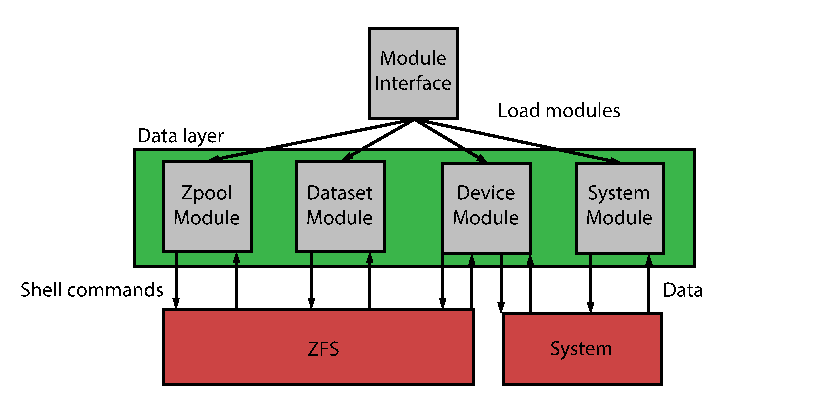
\includegraphics[scale=0.8]{datalayer.pdf}
        \caption{Datová vrstva aplikace}
        \label{datalayer}
    \end{figure}

    Nejobsáhlejším základním modulem je \verb|DatasetModule|, který poskytuje základní metody pro správu jednotlivých souborových systémů. Tento modul umožňuje administrátorovi vytvářet souborové systémy uvnitř poolu a libovolně je vnořovat. Dále nabízí možnost tyto souborové systémy ničit, upravovat a vytvářet jejich snapshoty. Informace o~souborových systémech shromažďuje a udržuje třída \verb|Dataset|, kterou tento modul využívá.

    Posledním implementovaným modulem je \verb|SystemModule|. Tento modul slouží ke shromažďování informací o~systémových prostředcích nebo pro získání informací o~operačním systému.

    Celková struktura datové vrstvy je představena na obrázku \ref{datalayer}, kde můžeme vidět jednotlivé moduly. Na obrázku je také vidět jak jsou jednotlivé moduly načítány pomocí třídy \verb|ModuleInterface|.

\section{Logická vrstva}
Hlavní vrstvou aplikace bude logická vrstva. Tato část bude mít za úkol provádět požadované akce na souborovém systému ZFS za pomoci ostatních vrstev aplikace. Data obdržená od datové vrstvy zpracuje a požádá prezentační vrstvu o~vygenerování HTML stránky. Výsledek je prostřednictvím webového serveru odeslán uživateli, který si ho pomocí webového prohlížeče může zobrazit.

Třídy logické vrstvy se obecně nazývají kontroléry. Kontroléry budou obsahovat metody, které budou představovat jednotlivé akce nabízené uživateli. Na základě směrování popsaného v~\ref{route} dojde k~dynamickému načtení kontroléru a vyvolání požadované metody. Volaná metoda přesně definuje, které moduly datové vrstvy budou načteny a jak obdržená data zpracuje.
    \subsection{Kontrolér}
    V~adresářové struktuře aplikace opět stanovíme adresář, kde najdeme jednotlivé definice kontrolérů. V~tomto případě veškeré zdrojové kódy tříd logické vrstvy najdeme v~adresáři \emph{app/controllers}.

    Právě odtud bude třída \emph{App}, která se stará o~směrování, dynamicky načítat požadované kontroléry. Stejně jako v~případě datové vrstvy nám dynamické načítání umožní načítat pouze ten kontrolér, který potřebujeme ke zpracování daného požadavku a opět ušetříme operační paměť.

    \subsection{Základní kontroléry}
    Do výsledné aplikace budou zařazeny následující kontroléry:
    \begin{itemize}
      \item \verb|DashboardConroller|
      \item \verb|DatasetConroller|
      \item \verb|DeviceConroller|
      \item \verb|ZpoolConroller|
    \end{itemize}

    Třída \verb|DashboardConroller| bude zajišťovat zobrazování úvodní stránky aplikace. Obsahem této stránky bude přehled základních informací týkajících se souborového systému obecně, vytvořených poolů nebo například všech dostupných souborových systémů.

    Stránky, které se týkají administrace souborových systémů v~ZFS, bude řídit třída \verb|DatasetConroller|. Tento kontrolér bude umožňovat zobrazit detailní informace o~jednotlivých souborových systémech a bude také nabízet funkce pro jejich administraci. Nebude tedy chybět možnost souborové systémy ničit, vytvářet, nastavovat nebo vytvářet jejich snapshoty.

    V~případě kontrolérů \verb|DeviceConroller| a \verb|ZpoolConroller| se bude jednat o~podobné funkce týkající se správy zařízení a ZFS poolů.

    Výsledná aplikace bude generovat HTML stránky, které v~sobě ponesou odkazy na metody výše zmíněných kontrolérů. Uživatel tedy vůbec nemusí znát strukturu aplikace a jednotlivé metody kontrolérů, protože mu budou nabídnuty prostřednictvím těchto stránek. Stránky mezi sebou budou logicky provázané tak, aby se uživatel mohl po aplikaci libovolně a pohodlně pohybovat.

    \begin{figure}
        \centering
        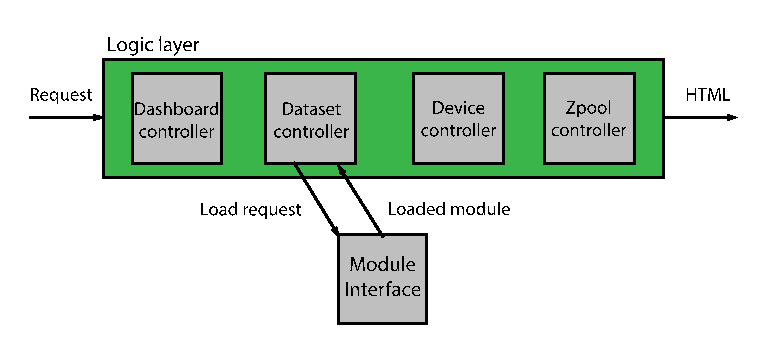
\includegraphics[scale=0.8]{logiclayer.pdf}
        \caption{Logická vrstva aplikace}
        \label{logiclayer}
    \end{figure}

    Struktura logické vrstvy aplikace je představena na obrázku \ref{logiclayer}, kde můžeme vidět jednotlivé kontroléry. Na obrázku je také znázorněno načítání modulů datové vrstvy pomocí třídy \verb|ModuleInterface|.

\section{Prezentační vrstva}
Poslední vrstvou aplikace je tzv. prezentační vrstva. Jediným úkolem této vrstvy je na základě obdržených dat vygenerovat požadovanou HTML stránku. Tato vrstva bude v~naší aplikaci zastoupena jedinou třídou \verb|BaseView|. Vzhledem k~dynamické povaze dat, které budeme v~aplikaci zobrazovat, využijeme šablonovací systém \emph{Jinja2} \cite{jinja2}, který je pro Python dostupný. Tento systém nám umožní vytvoření univerzálních šablon, které budou použity k~zobrazování více různých stránek. Stránka zobrazující detail souborového systému se bude vždy skládat ze stejných komponentů a bude mít stejné rozložení bez ohledu na to, jaký souborový systém právě zobrazujeme. Šabloně předáme data specifická pro konkrétní souborový systém a následně vygenerujeme výslednou HTML stránku.
    \subsection{Jinja2}
    Generování šablon ve třídě \verb|BaseView| je zajištěno pomocí modulu \emph{Jinja2}. Při vytváření instance této třídy dojde k~inicializaci tohoto modulu a stanovení adresáře, ze kterého se budou šablony načítat. Tento adresář se v~našem případě bude jmenovat \emph{template} a bude se nacházet v~kořenovém adresáři aplikace. Modul při každém požadavku na vykreslení šablony z~tohoto adresáře dynamicky načte potřebnou šablonu. Ta je následně vyplněna daty a vrácena jako textový řetězec.
    \subsection{Google charts}
    Pro demonstraci dynamického zobrazování dat v~HTML dokumentu využijeme jazyka JavaScript a technologie AJAX. Tato technologie nám umožní posílat HTTP požadavky z~již načtené stránky v~klientském webovém prohlížeči. V~požadavku klasicky specifikujeme požadovanou URL adresu a odešleme ho webovému serveru. Server zpracuje požadavek klasickým způsobem a odpoví klientovi. V~klientském prohlížeči data zpracujeme a dynamicky změníme část načtené stránky. Pro lepší práci s~JavaScriptem budeme využívat knihovnu jQuery \cite{jquery} a dynamická data budeme zobrazovat pomocí Google charts \cite{google}.

    Součástí implementované verze aplikace je funkce pro dynamické zobrazování procentuálního využití procesoru. Hlavním zdrojem dynamických informací o~systému je nástroj \emph{sar}.
    \subsection{Bootstrap}
    Designu webových stránek bylo dosaženo s~pomocí webového frameworku Bootstrap. Tento framework umožňuje rychlou tvorbu responzivních webových stránek. Hlavní důvod volby tohoto frameworku je možnost jednoduchého rozložení elementů stránky do řádků a sloupců \cite{bootstrap}.


\section{Rozšiřitelnost}
Výsledná aplikace je díky MVC architektuře a třídám, které zajišťují dynamické načítání komponentů, snadno rozšiřitelná.

Dynamické načítání logické vrstvy nám umožňuje přidat nově vytvořené třídy do adresářové struktury aplikace, bez nutnosti celou aplikaci restartovat. Pokud se požadovaná třída v~době požadavku v~aplikaci nenachází, jednoduše uživateli sdělíme, že stránka neexistuje. Pro rozšíření funkcionality stačí vytvořit novou třídu s~požadovanými funkcemi, která bude splňovat stanovené požadavky, a následně ji vložit do správného adresáře.

Jednotlivé moduly datové vrstvy jsou také načítány dynamicky, a proto můžeme datovou vrstvu rozšiřovat stejně lehce jako logickou. Vytvoříme modul podle struktury stanovené v~kapitole \ref{package} a vložíme ho do adresářové struktury aplikace. O~načtení nově vytvořeného modulu se aplikace postará sama.

\section{Startup}
Celá aplikace bude zaregistrována v~SMF, abychom docílili jednoduché manipulace s~aplikací. Pro registraci aplikace jako služby v~operačním systému si budeme muset vytvořit XML dokument, který jí bude popisovat. Dále budeme muset vytvořit tzv. start skript, který bude naši aplikaci ovládat. Nakonec pro úspěšný chod aplikace vytvoříme roli v~operačním systému Solaris, která bude mít práva provádět potřebné příkazy.
\subsection{Role}
Role se v~operačním systému Solaris vytvářejí pomocí příkazu \verb|roleadd|. Naše role se bude jmenovat \emph{wzfsadm} a nebude mít žádný domovský adresář. Nebudeme ji přiřazovat ani heslo. Tím dosáhneme toho, že se na ní bude moci přepnout pouze uživatel \emph{root} a nikdo jiný. Další výhodou je, že se na roli nedá přihlásit přímo při přihlašování do operačního systému, což omezuje některá bezpečnostní rizika.

Pomocí RBAC přiřadíme roli bezpečnostní profil, který bude sdružovat práva na vykonávání potřebných příkazů. V~systémovém souboru \emph{/etc/\-se\-cu\-ri\-ty/\-prof\_attr.d/\-core-os}, který obsahuje definice bezpečnostních profilů, vytvoříme nový profil \emph{wzfsadm}. Na tento profil se budeme odkazovat při vytváření práv na vykonávání příkazů v~souboru \emph{/etc/\-se\-cu\-ri\-ty/\-exec\_attr.d/\-core-os}. Na konec tohoto souboru vložíme seznam příkazů, které bude majitel tohoto profilu moci vykonávat s~identitou uživatele \emph{root}. Pro ukázku je zde uveden jeden řádek, který budeme přidávat na konec souboru s~právy.
\begin{verbatim}
wzfsadm:solaris:cmd:RO::/usr/sbin/zfs:euid=0
\end{verbatim}
V~prvním sloupci je název bezpečnostního profilu, ke kterému se právo vztahuje a v~předposledním sloupci je samotný příkaz. Poslední sloupec udává identitu, pod kterou bude příkaz spuštěn. Takto vytvořený profil s~právy přiřadíme roli pomocí příkazu \verb|rolemod|.
\subsection{Start skript}
Start skript bude umět aplikaci spustit, zastavit a restartovat. Jelikož jsme použili RBAC práva, bude tento skript napsaný v~tzv. profile shellu, který umí tyto práva interpretovat. Skript bude umět zpracovat parametry \emph{start}, \emph{stop} a \emph{restart}, které budou určovat prováděnou akci.

Při startu aplikace skript spustí soubor \emph{run.py}, který spustí webový server a celou aplikaci. Standardní výstup přesměruje do souboru \emph{default\_log} a chybový výstup do souboru \emph{error\_log}. Oba tyto soubory se budou nacházet v~adresáři \emph{/var/log/wzfsadm}, který bude sloužit pro uchovávání logů aplikace. V~závěru je uloženo PID spuštěného procesu do souboru, aby bylo později možné tento proces ukončit.

Zastavení aplikace znamená ukončení procesu webového serveru, jehož PID máme uložené v~souboru. Pro ukončení procesu je zavolán příkaz \verb|kill|.
\subsection{Manifest}
Manifest můžeme vytvořit například pomocí příkazu \verb|svcbundle|. Tento příkaz vygeneruje XML dokument, který bude naši službu popisovat. Jeho obsahem jsou především metody, které se budou provádět při zapínání a vypínání služby. Pro tento účel jsme vytvářeli výše zmíněný start skript, který použijeme jako metodu pro ovládání služby. Další součástí manifestu je tzv. kontext metody, který nám umožní specifikovat uživatele, pod kterým se bude celá služba spouštět. Zde uvedeme námi vytvořenou roli \emph{wzfsadm}. Posledním součástí je jméno služby, pod kterým budeme moci aplikaci spravovat. Součástí jména jsou i nadřazené kategorie, kterých se služba týká. V~našem případě bude jméno služby \emph{system/\-filesystem/\-wzfsadm}.

Následně zaregistrujeme službu pomocí příkazu \verb|svccfg import|, který přesune vytvořený manifest do adresáře \emph{/lib/\-svc/\-manifest} a restartuje službu \emph{manifest-import}, která se stará o~načítání jednotlivých manifestů.

Výhoda registrace služby v~systému spočívá v~jednoduchém ovládání pomocí příkazu \verb|svcadm|. SMF se také stará o~zaznamenávání chyb při manipulaci se službou. Administrátor se tedy může kdykoli podívat k~jaké chybě došlo.
\section{Balíčkovací systém}
Zdrojové kódy aplikace zabalíme pomocí nástroje \verb|pkgmk| do balíčku \emph{wzfsadm-i386.pkg}, který uživateli značně usnadní instalaci celé aplikace. Součástí balíčku budou i instalační skripty, které zajistí vytvoření role \emph{wzfsadm} s~potřebnými právy a také registrují službu \emph{wzfsadm} v~systému. Při odstranění balíčku dojde k~odstranění vytvořené role a služby spolu se všemi zdrojovými kódy aplikace.
\section{Testy}
Veškerý vývoj a testování probíhalo na operačním systému Solaris 11 verze 5.11, který byl spouštěn pomocí aplikace \emph{Virtualbox}. Hlavní výhodou aplikace \emph{Virtualbox} byla možnost přidávání disků do systému, bez nutnosti fyzické disky vlastnit. Stačí vytvořit virtuální disk v~hostitelském operačním systému a následně ho připojit k~virtuálnímu systému. Po startu systému je disk ihned k~dispozici.


